% Part: history
% Chapter: set-theory
% Section: limits

\documentclass[../../../include/open-logic-section]{subfiles}

\begin{document}

\olfileid[id]{his}{set}{limits}

\olsection{Definisi Limit yang Ketat}

Sekarang, penyelesaian standar bagi masalah di atas ialah menyingkirkan
infinitesimal. Berikut caranya.

Kita melihat bahwa ketika $\beta$ semakin kecil, kita memperoleh hampiran
gradien yang semakin baik. Bahkan, ketika $\beta$ mendekati $0$ sedekat apa
pun, nilai $f'(c)$ ``cenderung tanpa batas'' menuju gradien yang kita
inginkan. Jadi, alih-alih mempertimbangkan apa yang terjadi \emph{pada}
$\beta=0$, kita hanya perlu mempertimbangkan \emph{kecenderungan} $f'(c)$
ketika $\beta$ mendekati~$0$.

Dengan ungkapan ini, tantangan umumnya ialah memahami klaim berbentuk:
\begin{center}
Ketika $x$ mendekati $c$, $g(x)$ cenderung tanpa batas menuju $\ell$.
\end{center}
yang dapat kita tulis dengan lebih ringkas sebagai:
\[
\lim_{x \rightarrow c}g(x) = \ell.
\]
Pada abad ke-19, dengan mengembangkan karya Cauchy sebelumnya, Weierstrass
memberikan suatu definisi yang sepenuhnya ketat bagi ungkapan ini. Gagasannya
memang bahwa kita dapat membuat $g(x)$ sedekat yang kita inginkan
dengan~$\ell$ dengan membuat $x$ cukup dekat dengan~$c$. Lebih tepatnya,
kita menetapkan bahwa $\lim_{x \rightarrow c}g(x)=\ell$ berarti:
\[
(\forall\epsilon > 0)(\exists \delta > 0)\forall x
\left(0 < |x - c| < \delta \lif |g(x) - \ell| < \epsilon \right).
\]
Garis vertikal di sini menyatakan nilai mutlak. Artinya, $|x|=x$ jika
$x\geq0$, dan $|x|=-x$ jika $x<0$; fungsi \emph{tersebut} dapat digambarkan
sebagai berikut:
\begin{center}
	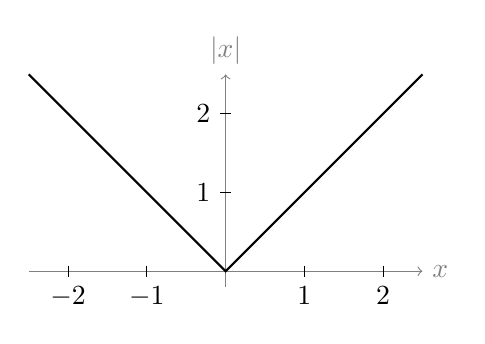
\begin{tikzpicture}[scale=1]
	\draw[->, gray] (-2.5,0) -- (2.5,0) node[right] {$x$};
	\draw[->, gray] (0,-.2) -- (0,2.5) node[above] {$|x|$};

	\foreach \x/\xtext in {-2/-2, -1/-1, 1/1, 2/2}
	\draw[shift={(\x,0)}] (0pt,2pt) -- (0pt,-2pt) node[below] {{$\xtext$}};

	\foreach \y/\ytext in {1/1, 2/2}
	\draw[shift={(0,\y)}] (2pt,0pt) -- (-2pt,0pt) node[left] {{$\ytext$}};

	\draw[thick] (-2.5, 2.5)--(0,0)--(2.5, 2.5);
	\end{tikzpicture}
\end{center}
Jadi, secara kasar definisi itu mengatakan: Anda dapat membuat
``galat'' lebih kecil daripada $\epsilon$ (yakni
$|g(x)-\ell|<\epsilon$) dengan memilih argumen yang tidak sama dengan $c$
dan berjarak kurang dari $\delta$ dari~$c$ (yakni
$0<|x-c|<\delta$).

Setelah mendefinisikan pengertian limit, kita dapat menggunakannya untuk
sepenuhnya menghindari infinitesimal dengan menetapkan bahwa gradien $f$
pada $c$ diberikan oleh:
\[
	{f}'(c) = \lim_{x \rightarrow 0}
	\left(\frac{f(c +x) - f(c)}{x}\right)
	\text{ jika limitnya ada}.
\]
Namun, penting untuk memahami mengapa definisi kita memerlukan syarat
``jika limitnya ada''. Sebagai contoh sederhana, pertimbangkan
$f(x)=|x|$, yang grafiknya baru saja kita lihat. Jelas bahwa $f'(0)$ tidak
terdefinisi dengan baik: jika kita mendekati $0$ ``dari kanan'',
gradiennya selalu $1$; jika kita mendekati $0$ ``dari kiri'', gradiennya
selalu $-1$; jadi, limitnya tidak terdefinisi. Dengan demikian, kita dapat
menambahkan bahwa suatu fungsi~$f$ \emph{dapat didiferensialkan} pada~$x$
jika dan hanya jika limit tersebut ada.

Kita telah melihat cara menangani diferensiasi dengan menggunakan pengertian
\emph{limit}. Kita dapat menggunakan pengertian yang sama untuk
mendefinisikan gagasan fungsi \emph{kontinu}. (Pada hakikatnya, Bolzano
telah menyadarinya pada 1817.) Perlakuan Cauchy--Weierstrass terhadap
kontinuitas adalah sebagai berikut. Secara kasar, suatu fungsi~$f$ kontinu
(pada suatu titik) jika, ketika Anda menuntut tingkat ketelitian tertentu
pada keluaran fungsi, tuntutan itu dapat dijamin dengan mengharuskan tingkat
ketelitian tertentu pada masukan fungsi. Lebih tepatnya, $f$ kontinu pada
$c$ jika, ketika $x$ cenderung ke nol, selisih antara $f(c+x)$ dan $f(c)$
sendiri cenderung ke~$0$. Dengan kata lain, $f$ \emph{kontinu} pada $c$
jika dan hanya jika
$f(c)=\lim_{x\rightarrow c}f(x)$.

Melangkah lebih jauh hanya akan membawa kita ke analisis real, padahal pokok
bahasan kita ialah teori himpunan. Jadi, sekarang kita perlu berhenti dan
menyatakan pelajarannya. Selama abad ke-19, para matematikawan belajar
bekerja tanpa infinitesimal dengan menggunakan pengertian \emph{limit} yang
didefinisikan secara ketat.

\end{document}
